\chapter{System Modeling}

"A dynamic system is a system that change or evolve over time \cite{CTMS2019_Modeling}. Dynamic systems can be represnted generally by either \textbf{First Order} or \textbf{Second Order} differential equations. In general a system can be represented in a state equation form as:
\begin{equation}
	\begin{bmatrix}
	\dot{x}
	\end{bmatrix} = f (\begin{bmatrix}
	x(t)
	\end{bmatrix},\begin{bmatrix}
	u(t)
	\end{bmatrix}, t )
\end{equation}

where,
\begin{itemize}
	\item $\vec{\dot{x}}$ is a vector of dynamics (rate of change) of the states of the system
	\item $\vec{x(t)}$ is the vector of states of the system
	\item $\vec{u(t)}$ is the vector of inputs to the system
\end{itemize}

From the initial conditions of the states $x_0$ at $t = 0$, and the history of the inputs $u(t)$ the next possible states value after every time step can be determined both analytically or through numerical integration.

\textbf{Assumptions}

A nonlinear time dependent function is generally difficult to solve mathematically, so two assumptions are made in order to simplify the problem statement.

\begin{enumerate}
	\item If $f$ does not depend on time explicitly such as that $\dot{x} = f(x(t),u(t))$ instead of $\dot{x} = f(x(t),u(t),t)$, then the system is said to be time-invariant. The state variables $x(t)$ and the control inputs $u(t)$ may still be dependent on time. Also for time-invariant systems, the parameters or the coefficients of the function $f$ are constant \cite{CTMS2019_Modeling}.
	\item An explicit function in mathematics is a function that can be written in the form: $y = f(x)$ such as $y = 5x^3 - 3$, in case of time-invariant functions which can be written in a form $y = e^{at}$ which is not a time-explicit function. $a$ is a coefficient that is a constant, there are time-varying coefficients such as $\sin{\alpha}$. When the systems are not dependent on time explicitly, physically their behavior does not change with time, such that once the step response of a spring-mass system reaches its steady-state value, the response wont change after a certain amount of time has been passed.
	\item Systems can be assumed a linear behavior over a certain range of their operation. In such a case, the differential equation that represents the dynamics can be expressed in a linear matrix form $\dot{x} = Ax + Bu$.
\end{enumerate}

\section{Three phase method of modeling} \label{Sec_ThreePhaseModeling}

A three phase method is employed for modeling a system using mathematical relationships as follows

\begin{enumerate}
	\item Structuring
	\begin{enumerate}
		\item Divide complex system into subsystems
		\item Establish the input output relationship between various subsystems that can be connected together such as using TF's of every subsystem block
	\end{enumerate}
	\item Use first principles from physics
	\begin{enumerate}
		\item Conservation laws: Conservation laws are the balance equations established using the first principles of physics, most of the commonly used balance equations from physics are as follows
		\begin{enumerate}
			\item Force balance (Newtons Laws for linear motion)
			\item Torque balance (Newton's Laws for angular motion)
			\item Voltage balance (Kirchhoff's voltage law)
			\item Current balance (Kirchhoff's current law)
			\item Volume flows (Fluid flow modeling)
		\end{enumerate}
		\item Constitutive relations: These relations relate variables of different units with each other or some quantity such as
		\begin{enumerate}
			\item Ohm's Law (Relates voltage across an electrical component to the current flowing)
			\item Ideal gas law (Relates relationship between pressure, volume and temperature of gas molecules)
			\item Hooke's Law (Relates relationship between displacement and force of a spring)
			\item Air resistance (between velocity of the air and force exerted by it on a cross sectional area)
		\end{enumerate}
	\end{enumerate}
	\item Equations put together in a standardized way for analysis, simulation and design
	\begin{enumerate}
		\item Here using State-space method, as it is a modern design concept and has advantages modeling complex systems and their control design over classical control methods
		\item State-space method uses the following method in general
		\begin{enumerate}
			\item $\dot{x} = f(x,u,d)$, the evolution of a state variables is a function of the states $x$ itself, the inputs $u$ and disturbances to the system $d$
			\item the output $y = h(x,u,d)$ is another function of the states $x$, the inputs $u$ and disturbances while measuring $d$
			\item An easy way to choose state variables is to ask: What is the variable in formed equations from phase II that is changing (Hint: Check the variables that are written in time derivatives and start from there). As state-space model is not unique, any other new chosen variable would change model and express the new model with reference to new variable.
		\end{enumerate}
	\end{enumerate}
\end{enumerate}

In order to illustrate the above modeling method consider a mechanical system of a simple mass-spring system. 
\subsubsection{Phase I: Subsysteming and choosing inputs and outputs}

For the first phase the input can be recognized as $F(t)$ and output as $x(t)$, therefore the subsystem is a system that transform the input $F(t)$ to displacement $x(t)$.

\subsubsection{Phase II: Mathematical modeling}

In the second phase the following questions are asked
\begin{itemize}
	\item What is it that changes?
	\item What is causing this change?
\end{itemize}
For the case of spring-mass system, both these questions are answered using Newton's Law which relates the motion (effect) in terms of forces (cause) acting on the system using
\begin{equation}
	\sum F_{net} = m \ddot{x} \implies F_{ext} - F_{int} = m \ddot{x} \implies  F_{ext} - F_{spring} = m \ddot{x}
\end{equation}
Finally, the constitutive relationships for the spring force needs to be established, here using Hooke's law
\begin{equation}
	F_{spring} = K x
\end{equation}
The equations formed using physics can be put together, which forms a compact form of system description expressed mathematically
\begin{equation} \label{Eq_Modeling_MechanicalSystems}
	F_{ext} - K x = m \ddot{x}
\end{equation}
In the third phase, these equations has to be put together (in this case using a state-space model) so as to render its analysis, simulation and design of components (redesigning or control design).

\subsubsection{Phase III: Writing State-space form}

Looking at equations of motion formed using Phase II, it can be seen that the variable that is changing and the one that has time derivative term in equation \eqref{Eq_Modeling_MechanicalSystems} is $\ddot{x}$. State-space forms are always to be written in first order differential or difference equations form. Therefore, further structuring is required using new variables so as to split a second order ODE to a system of two first order ODE's.
\begin{align}
	y &= x \\
	\dot{y} &= \dot{x}
\end{align}
The state derivatives can now be expressed as
\begin{align}
	\frac{dy}{dt} &= \dot{x} \\
	\frac{\dot{y}}{dt} &= \ddot{x} = \frac{F_{ext}}{m} - \frac{Ky}{m} \label{Eq_Modeling_StspEquationFrom}
\end{align}
It can be seen that equation \eqref{Eq_Modeling_StspEquationFrom} is written in the form of $\dot{x} = f(x,u,d)$ where the derivative of state-variable is a function of the states $x$ itself, the inputs $u$ and disturbances to the system $d$ (in this case there is no $d$).

\section{Model verification and validation}

Verification is the process of determining that the model implemented is accurate. That is, it is a check if the implementation (software, computer code) represents the mathematical model accurately according to the developers conceptual description and the solution to the model

Validation is the process of determining the degree to which a model is an accurate representation of the real world from the perspective of the intended uses of the model (check to see if all use case scenarios are matched)

\begin{figure}[h!]
	\centering
	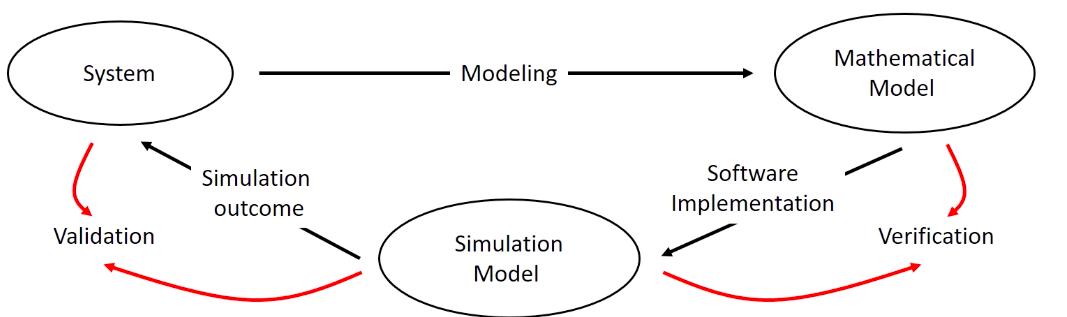
\includegraphics[width=\linewidth]{Bilder/Model_Verification_Validation}
	\caption{Model verification and validation definition}
	\label{Fig_ModelVerificationValidation}
\end{figure}
\newpage

\section{Mathematical Modeling}

In mathematical modeling of the dynamic systems, there are two approaches. State space approach and Laplace transform (or writing the transfer function) of the system. 

\subsection{State Space Representation}

In state space approach the linear time-invariant (constant coefficient) first order differential equation can be written as a linear sum of matrices containing the dynamic states and the control inputs to the system. 

For continuous linear time-invariant (LTI) systems, the standard form of state-space representation is \cite{CTMS2019_Modeling}:

\begin{align}
	\dot{x} &= Ax + Bu\\
	y &= Cx + Du
\end{align}

\begin{itemize}
	\item $\dot{x}$ is the system dynamics
	\item if $u(t)$ is input to the system
	\item Any measured output should also be a function of $x(t)$ plus $u(t)$.
	\item Matrix $A$ defines the system matrix, that is the coefficient of all system states.
	\item Similarly, matrix $B$ represents the coefficients of all system inputs.
	\item Equation $y(t)$ is the output of the system that is of control importance.
	\item Matrix $C$ is used to choose the states that are required for control, other non-important states from the controls point can be ignored.
	\item Matrix $D$ is used to choose the inputs that directly influence the outputs, otherwise $D$ is taken as zero matrix.
\end{itemize}

\section{Transfer function representation}

With transfer function representation, the linear ordinary differential equation representing the dynamics of the states can be transformed into a linear algebraic equation. Laplace transform is conducted to transform a function $f(t)$ from time domain to a $s$ domain. A $s$ domain is a domain of complex numbers $s = \sigma \pm j \omega$ which are plotted on the complex plane of real and complex numbers. The transfer is performed through the function $$ \int_{0}^{t} e^{-st} f(t) dt $$. A $s$ domain is a plane of complex numbers, where the solution of the transfer function can be plotted and studied easily. It so happens that for a system such as a mass-spring with a damper, the real plane values control the damping and the imaginary values control the frequency of the system respectively. $s$ domain is not a transformation to a frequency domain rather to a domain of complex numbers that are easier to evaluate and visualize.

\textit{Transfer functions model only linear systems.}

\textit{More detailed mathematical derivations are provided in one note notes}.

\section{General form of Second order System}

Consider a PT-2 system such as a mass, spring and a damper system which can be written in the form as:
\begin{equation}
m \ddot{x} + k \dot{x} + c x = 0
\end{equation}
division by $m$ on both sides:
\begin{equation*}
\ddot{x} + \frac{k}{m} \dot{x} + \frac{c}{m} x = 0
\end{equation*}
Following substitutions can be made using system parameters as given below:
\begin{align*}
\frac{k}{m} &= 2 \delta \\
\frac{c}{m} &= \omega_{n}^{2}
\end{align*}
where $\delta$ is called the damping coefficient (how fast the oscillations damp out?) and $\omega_{n}$ is called the natural or Eigen frequency of the undamped system (how fast does the undamped system oscillate?). Therefore, the above equation becomes:
\begin{equation}
\ddot{x} + 2 \delta \dot{x} + \omega_{n}^2 = 0
\end{equation}
Further, a new term damping ratio can be defined as $\zeta = \delta / \omega_{n}$ with $\delta$ the damping coefficient of the system. Therefore, the above equation can be re-written as:
\begin{equation}\label{Eq_GeneralFrom_PT2}
\ddot{x} + 2 \zeta \omega_{n} \dot{x} + \omega_{n}^2 = 0
\end{equation}
Using equation \eqref{Eq_GeneralFrom_PT2}, general form of PT-2 non-homogeneous systems can be expressed as:
\begin{equation} \label{Eq_PT2_system}
\ddot{y}(t) + 2 \zeta \omega_{n} \dot{y}(t) + \omega_{n}^{2} y(t) = \omega_{n}^{2} u(t)
\end{equation}

Once a general form of PT-2 system is obtained then in the literature there are various ways to solve them using methods such as Laplace transform as described in section \ref{Sec_Solving_PT2_Laplace}, Algebraic (Eigen-Value analysis) as described in section \ref{Sec_StabilityLinearSystems} and Numerical (Matlab). All these methods are aimed primarily at determining the modes of motion that the PT-2 system exhibits and thereby determine its stability.

\section{Non-Canonical Systems}

Non-canonical systems are the ones that do not fit into the domain of first and second order systems. They are generally of the following types:
\begin{enumerate}
	\item Higher order systems (more than two poles)
	\item Nonlinear systems
	\item Systems with zeros ($s$ terms in the numerator)
\end{enumerate}

\subsection{Higher order systems}

In general the response of the higher order systems can be considered as the sum of first and second order responses. The exact time reponses can be determined using partial fraction expansion in Laplace domain. The poles themselves can have only real roots or complex conjugates, with such a limited possibility it is easier to then map the responses of the higher order systems with the responses learnt from such roots in the first and the second order systems. For example a higher order system can be expressed in Laplace domain as follows:
\begin{equation}
	\frac{K}{(s+a) (s^2 + \zeta \omega_{n} s + \omega_{n}^2)} = \frac{A}{s+a} + \frac{B}{s^2 + \zeta \omega_{n} s + \omega_{n}^2)}
\end{equation}
Additionally, most of the higher order system reponses can be approximated with either the first or the second order responses. This is either because of dominant roots of first or second order type which would domainate the response of the system (approximating the overall behavior) or because of the system behavior in terms of component or subcomponent level where the states exhibit the reponse of canonical systems (as in the case of a vaccum tube which is very nonlinear in its response in the component levels but linear in its higher subsystem level).

\subsubsection{Model reduction}

This section provides some ideas on model reductions of higher order systems. One of the techniques used in model reduction is to split the higher order terms into simple components of first and second orders working as components or subsystems for the entire system of the higher order. An example:
\begin{equation}
	G(s) = \frac{Y(s)}{U(s)} = \frac{20}{(s+2)(s+10)}
\end{equation}
Such a higher order system can be replaced with a components of first order systems connected in series such as:
\begin{equation} \label{Eq_ModelReduced_Eq}
	 \frac{20}{(s+2)(s+10)} = \frac{2}{s+2} \cdot \frac{10}{s+10}
\end{equation}
this is not partial fraction expansion of transfer function (required to solve for the coefficients) and cannot be performed using Matlab, rather this is just a simple splitting of the subsystem into components \textbf{\textit{connected in series}}. Also, this operation cannot be performed on electrical circuits though they are connected in series as circuit have cascading effects (the later components load onto the former components). This system now has two poles at $s = -10$ and $s = -2$ in which case the response of the system can be determined as settling time using these two poles as $e^{-10t}$ and $e^{-2t}$ ($e^{\sigma t}$ would be a possible analytical solution for a first order ODE). Also noting that the system has only real poles therefore, it signifies damping in the system. Here the component with response $e^{-10t}$ is much quicker than component with $e^{-2t}$ as the response will be equal to $t_s = \sigma/10$ and $t_s = \sigma/2$ respectively.

Using Matlab it can be seen that the response time of the system becomes quicker with increasing the damping ratio $\zeta$. As $\zeta$ is doubled and quadrupled from $\zeta = 0.2$ to $\zeta = 0.4$ and $\zeta = 0.8$, though the damping the higher the response times would also become more quicker which also doubles and quadruples as given by the real part of the poles from $s_{1,2} = -1$ to $s_{1,2} = -2$ and $s_{1,2} = -4$. Therefore, higher damping ratios $\zeta$ will make the system responses much quicker this will greatly reduce the period of the oscillation and therefore it will not be comforting experience when used as shock absorbers in vesicles. Another thing to note is that the damping ratio $\zeta$ does not change the steady state step response at all, it only changes the settling time $t_s$ taken by the system to reach the steady state as shown in the figures (\ref{Fig_stepResponsez_02}, \ref{Fig_stepResponsez_04} and \ref{Fig_stepResponsez_08}).
\begin{figure}[h!]
	\centering
	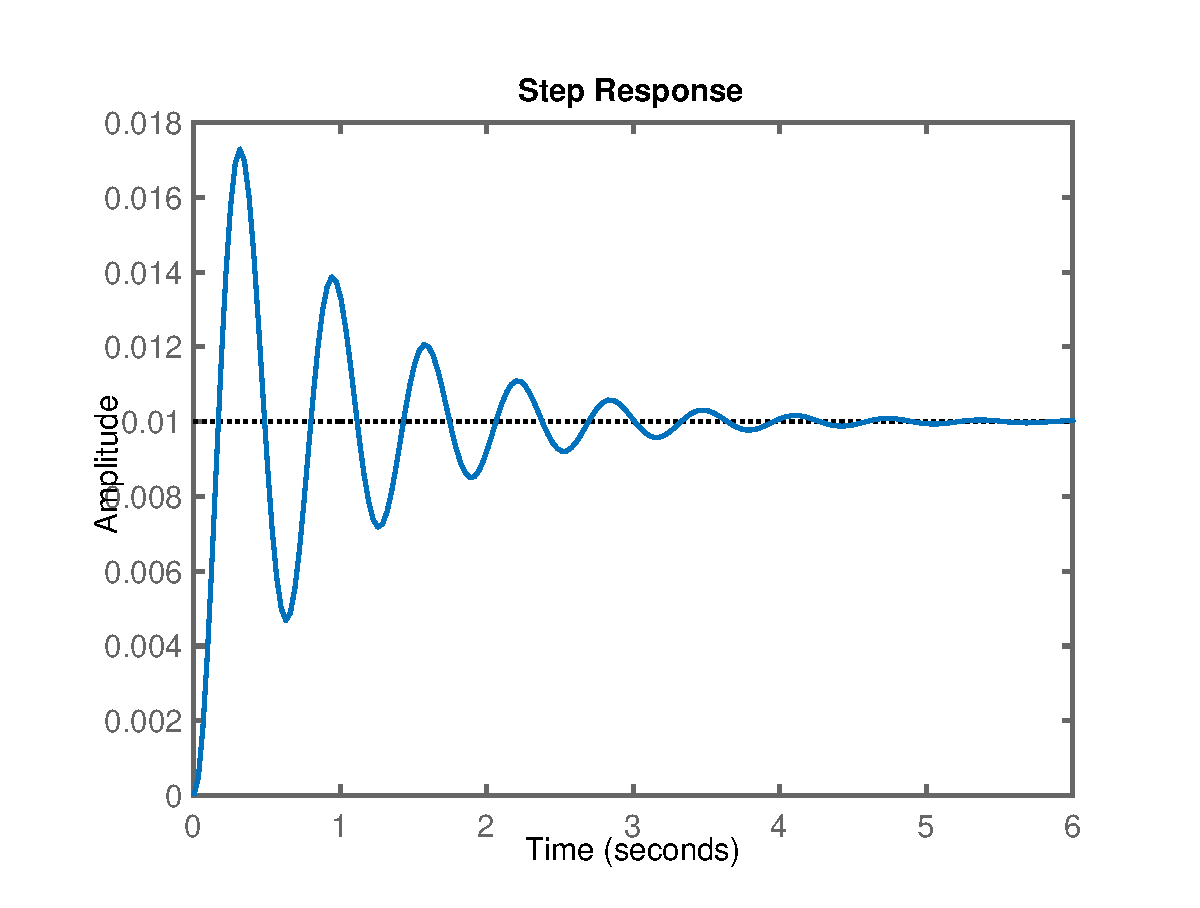
\includegraphics[width=0.5\linewidth]{Bilder/stepResponsez_02.eps}
	\caption{Step response at $\zeta = 0.2$}
	\label{Fig_stepResponsez_02}
\end{figure}
\begin{figure}[h!]
	\centering
	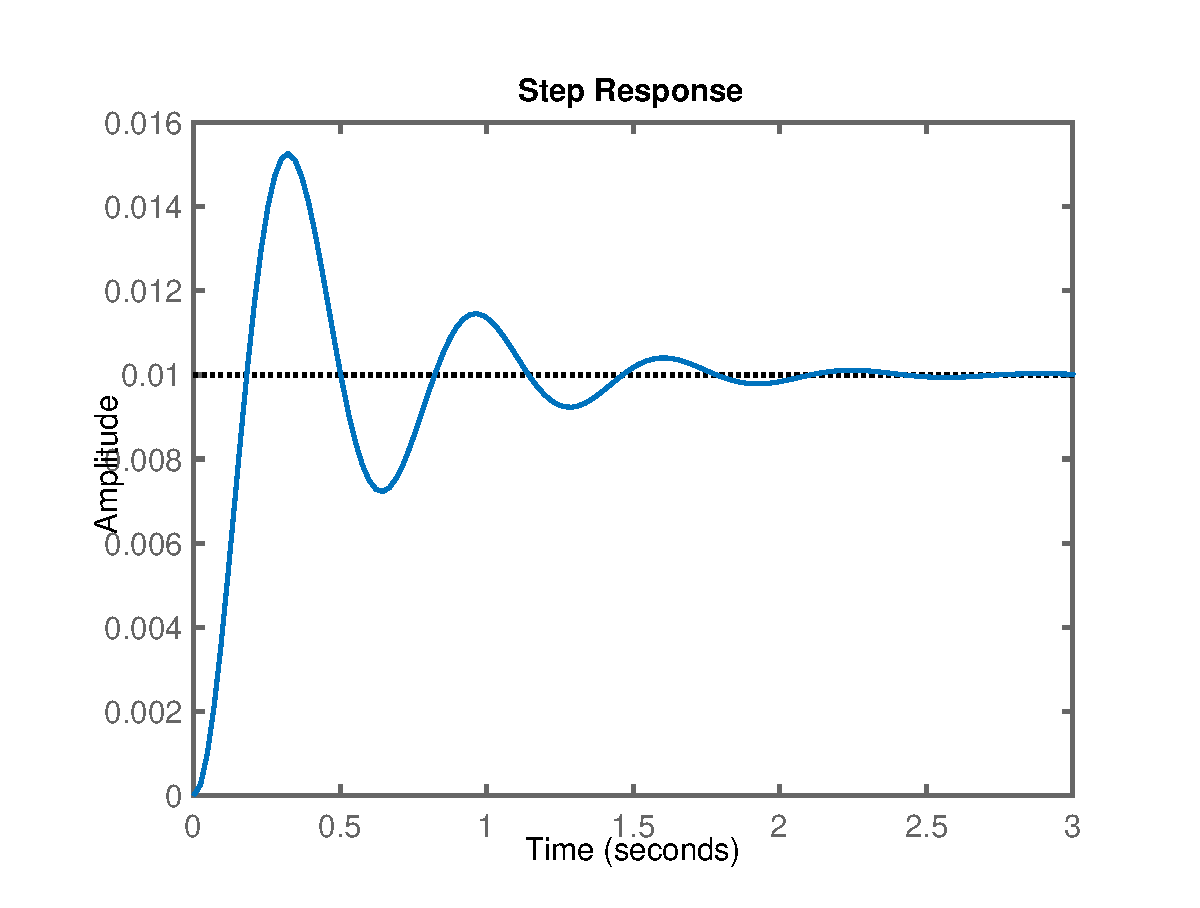
\includegraphics[width=0.5\linewidth]{Bilder/stepResponsez_04.eps}
	\caption{Step response at $\zeta = 0.4$}
	\label{Fig_stepResponsez_04}
\end{figure}
\begin{figure}[h!]
	\centering
	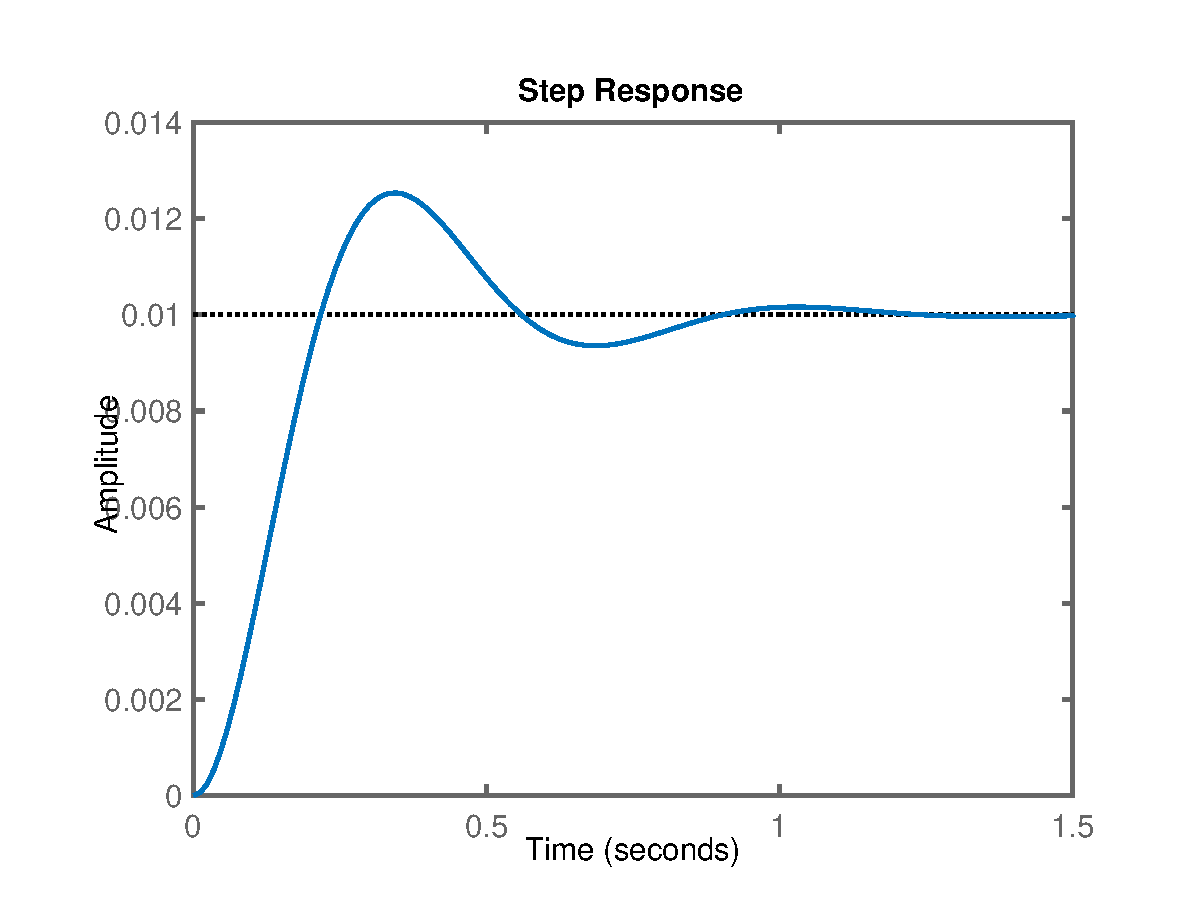
\includegraphics[width=0.5\linewidth]{Bilder/stepResponsez_08.eps}
	\caption{Step response at $\zeta = 0.8$}
	\label{Fig_stepResponsez_08}
\end{figure}
\clearpage
Going back to the example given by equation \eqref{Eq_ModelReduced_Eq}, the responses of the individual components can be plotted using Matlab as shown in figures \ref{Fig_MOR_E1_C1_step} and \ref{Fig_MOR_E1_C2_step}:
\begin{figure}[h!]
	\centering
	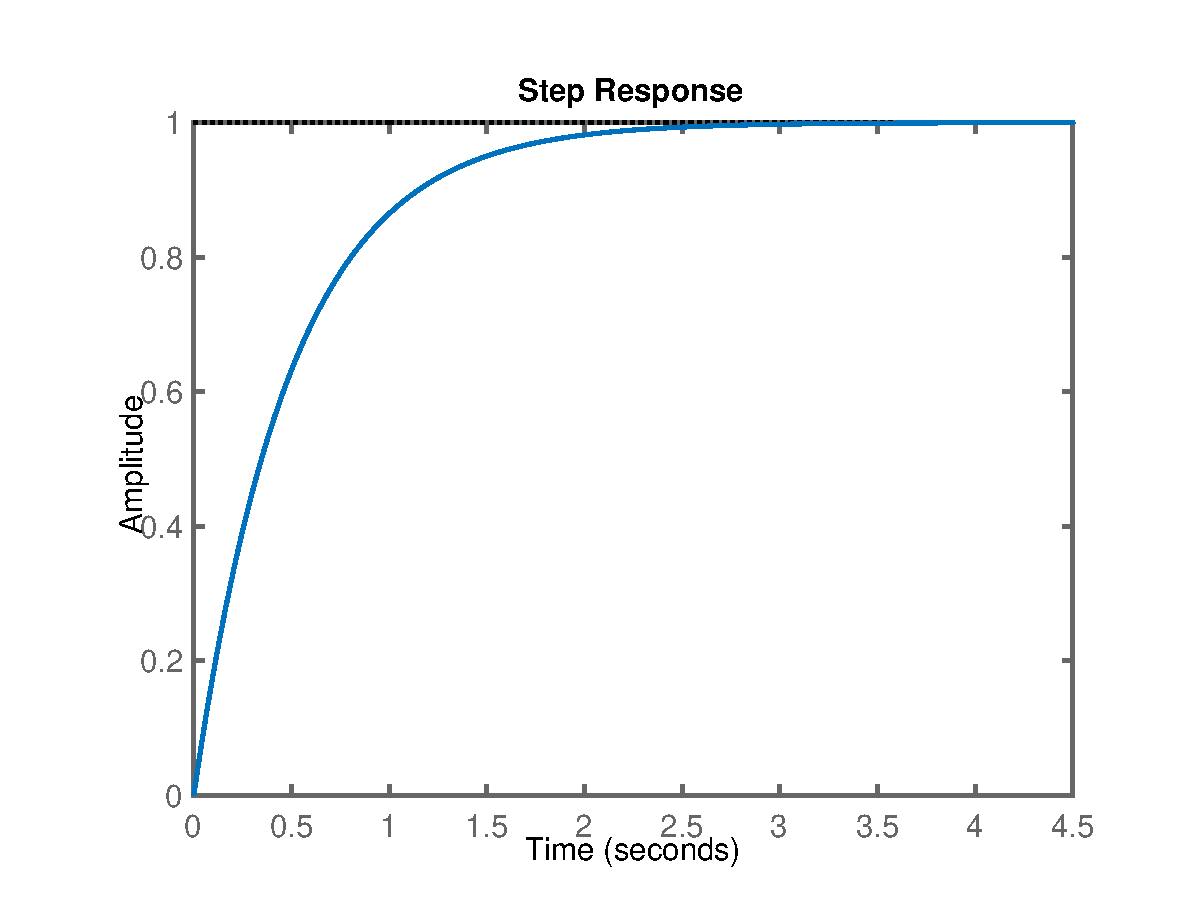
\includegraphics[width=0.7\linewidth]{Bilder/MOR_E1_C1_step.eps}
	\caption{Step response for pole at $s = -2$}
	\label{Fig_MOR_E1_C1_step}
\end{figure}
\begin{figure}[h!]
	\centering
	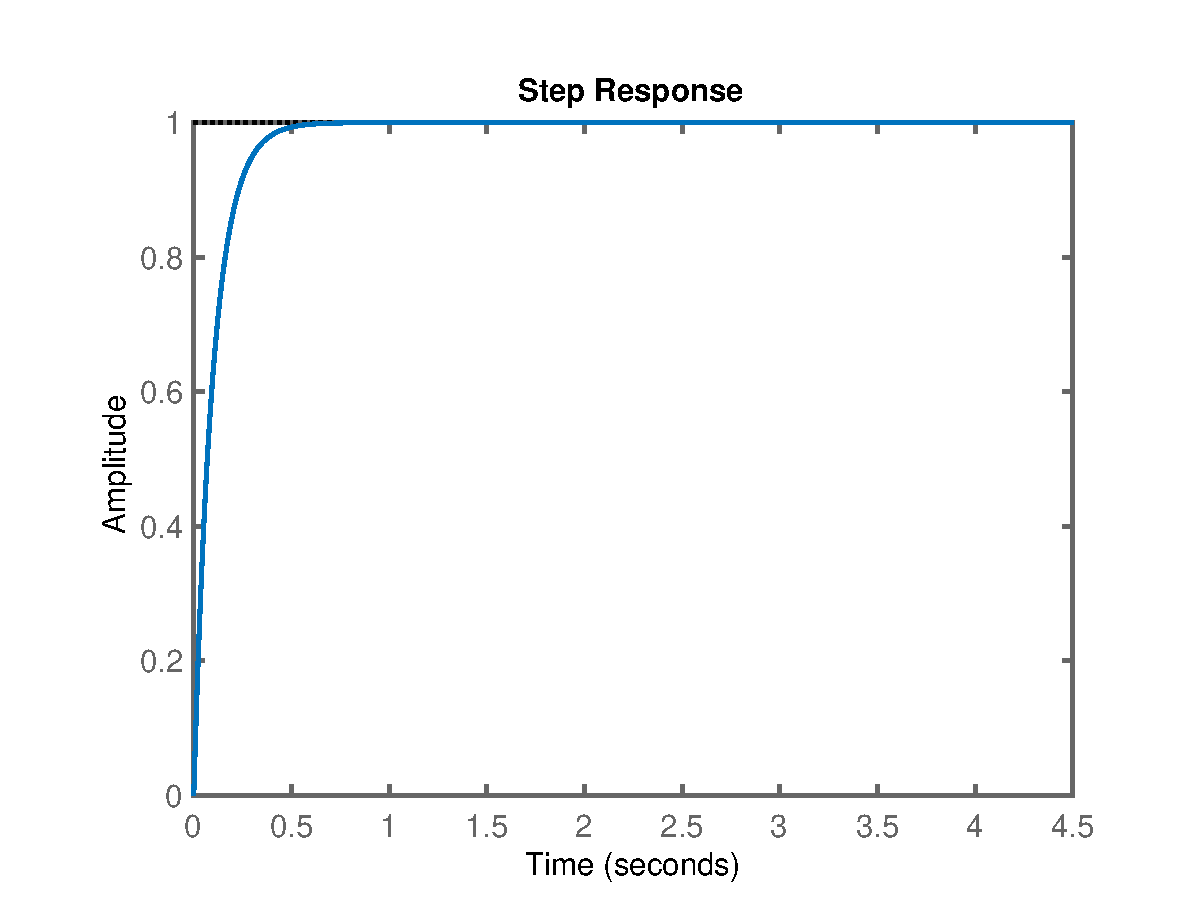
\includegraphics[width=0.7\linewidth]{Bilder/MOR_E1_C2_step.eps}
	\caption{Step response for pole at $s = -10$}
	\label{Fig_MOR_E1_C2_step}
\end{figure}
\clearpage
It can be seen clearly from figures (\ref{Fig_MOR_E1_C1_step} and \ref{Fig_MOR_E1_C2_step}) that the response of the system is much higher at higher damping ratios and this does not change the step response of the system itself. Generally since the response of component with response $e^{-2t}$ will be much slower it will dominate the overall system behavior as this makes the entire system as slow as response $e^{-2t}$ is. Consider figure \ref{Fig_MOR_E1_S_step}, which shows the response of the whole system with both the poles $s_{1,2} = \{ -2,-10 \}$
\begin{figure}[h!]
	\centering
	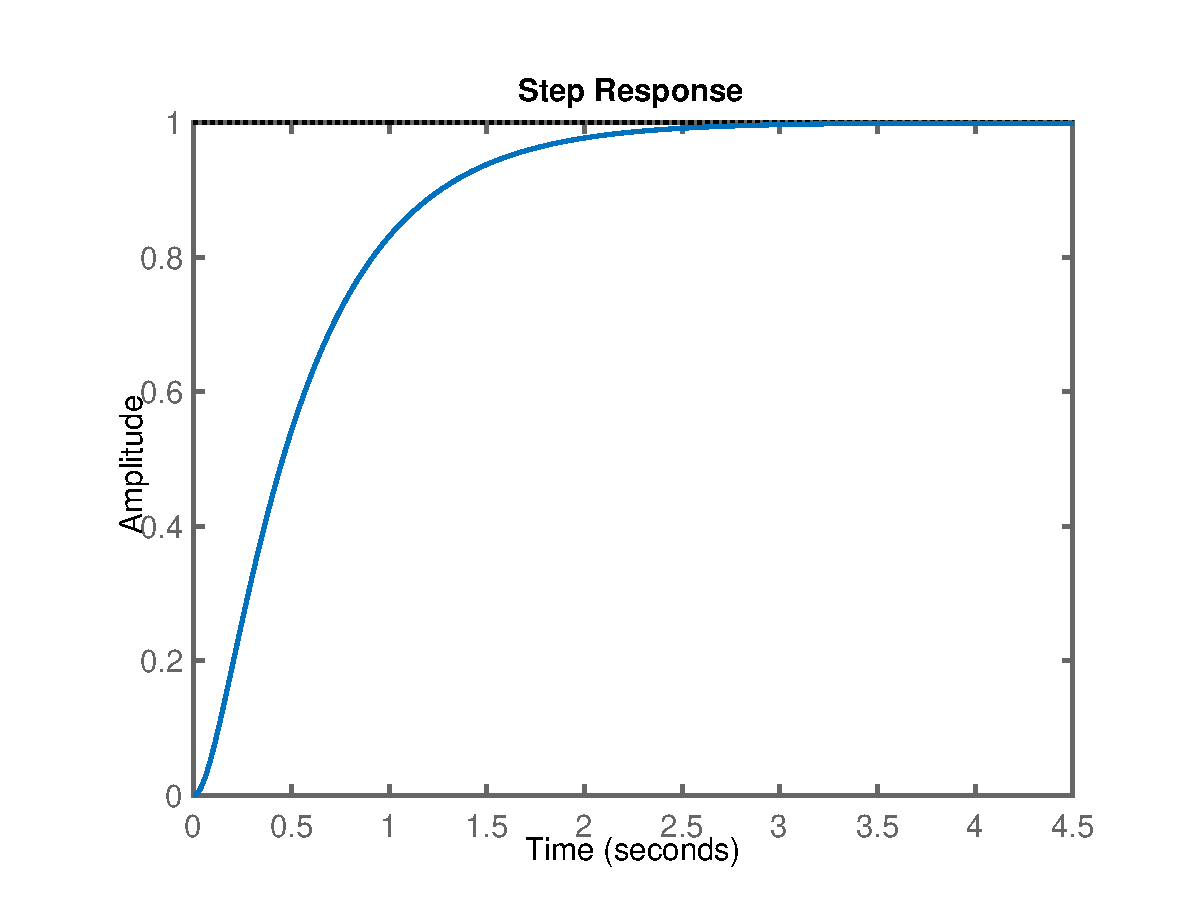
\includegraphics[width=0.7\linewidth]{Bilder/MOR_E1_S_step.eps}
	\caption{Step response for whole system with both the poles at $\{ -2,-10 \}$}
	\label{Fig_MOR_E1_S_step}
\end{figure}
It can be seen from figure \ref{Fig_MOR_E1_S_step} that the response of the system as a whole and the response of the system with only one component with pole at $s = -2$ is almost the same. Therefore, such techniques can be used to reduced the size of a higher order model by approximating the behavior to a lower order systems. 

In such a case the response of the component with response $e^{-10t}$ have almost no influence on the system, however, care has to be taken to include its steady state contribution which can be done just by using a static gain $K$ in Simulink. The size of $K$ depends on the value of the step function (DC gain from the faster component) that goes as an input to the slower component. For example if the step response (of a faster component) is of magnitude $1$, then a static gain of $K = 1$ will be given as input to the slower component. In general the gain that is needed to replace into the reduced system can be found using \textbf{\textit{final value theorem}}. Consider the system given by equation \eqref{Eq_ModelReduced_Eq}, the gain of the system can be given by:
\begin{equation}
	G(s) = \frac{20}{(s+2)(s+10)} \approx G_{Red}(s) = \frac{K}{s+2}
\end{equation}
here gain $K$ has to be set such that $G(s)$ and $G_{Red}(s)$ are both the same. $K$ or DC gain of a system is defined as \textbf{\textit{the steady-state response of the system for a DC input}} (constant input) such that:
\begin{equation}
	k_{dc} = lim_{s \rightarrow 0} s Y(s)
\end{equation}
where $$Y(s) = G(s)U(s) = \frac{20}{(s+2)(s+10)} \frac{1}{s}$$
therefore,
$$ k_{dc} = lim_{s \rightarrow 0} s \frac{20}{(s+2)(s+10)} \frac{1}{s} = lim_{s \rightarrow 0} G(s) = G(0) $$
$k_{dc}$ for the original system given by equation \eqref{Eq_ModelReduced_Eq} can be found therefore as follows:
\begin{equation}
	G(0) = \frac{20}{(0+2)(0+10)} = 1
\end{equation}
A $k_{dc} = 1$ will produce a steady-state value of $G(0) = 1$ for the system. Therefore, the DC gain of the reduced system should be $k_{dc} = 1$, such that:
\begin{equation}
	G_{Red}(s) = \frac{1}{s+2}
\end{equation}

\subsection{Effect of zeros}

\textbf{Zeros} are the values of $s$ that make the numerator of the transfer function $G(s)$ go to zero. They are the counterparts of poles. There effect on the poles can be studied using partial fraction expansion in Matlab using the command \textbf{\textit{[C,p] = residue(20,[1 12 20]);}}. 
\subsubsection{Effect 1: Contribution of each pole to the transfer function}
Consider the original system with no zeros and its partial fraction expansion:
\begin{equation}
	G(s) = \frac{20}{(s+2)(s+10)} = \frac{2.5}{s+2} - \frac{2.5}{s+10}
\end{equation}
now with zeros induced into the system the partial fraction expansion:
\begin{equation}
	G(s) = \frac{s+20}{(s+2)(s+10)} = \frac{2.25}{s+2} - \frac{1.25}{s+10}
\end{equation}
zeros effectively change the coefficients of the transfer function ie., they change the contribution of the poles on $G(s)$.
\subsubsection{Effect 2: Increases the overshoot}
Consdier the explanation given in figure \ref{Fig_EffectofZeros2}:
\clearpage
\begin{figure}[h!]
	\centering
	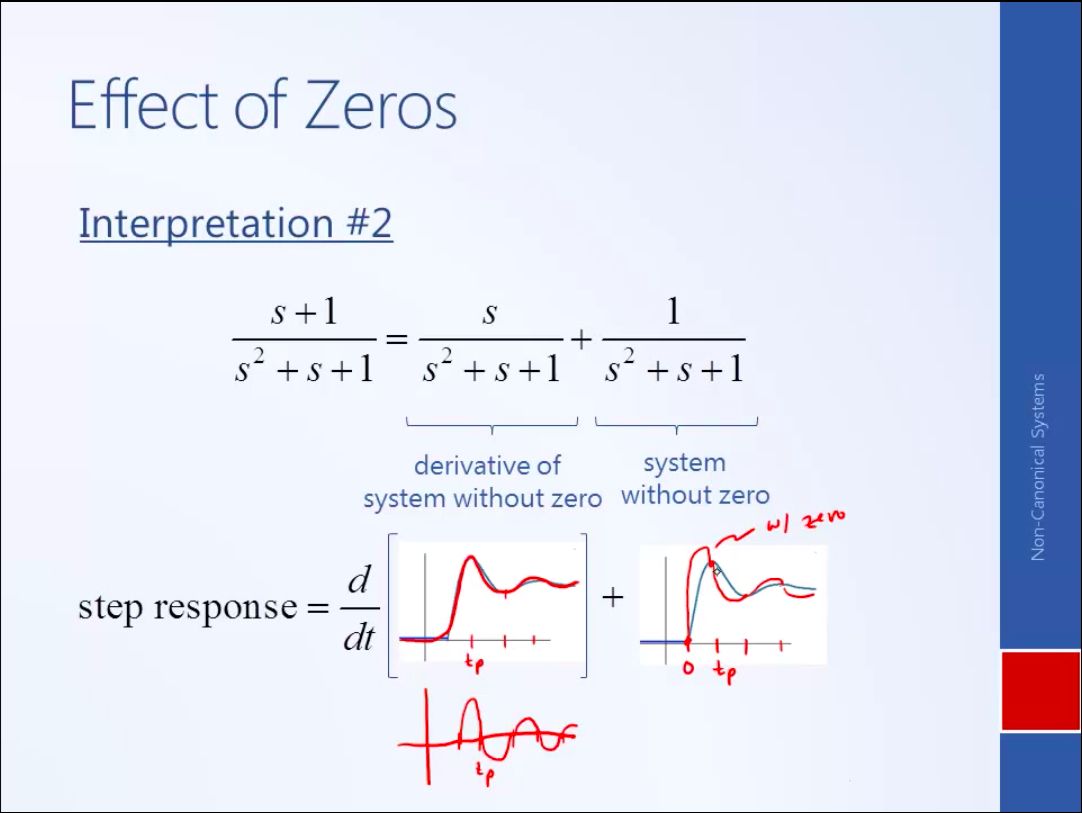
\includegraphics[width=\linewidth]{Bilder/Effect_of_Zeros_2}
	\caption{Zeros increase the overshoot of the system}
	\label{Fig_EffectofZeros2}
\end{figure}
As multiplication of $s$ to a transfer function is considered derivative we have a first term in the equation that the derivative of the step response. Adding the derivative part will carry the values of the derivatives to the step response which will increase the overshoot of the system as shown in figure \ref{Fig_EffectofZeros2}. Further consider figure \ref{Fig_EffectofZeros2_2}, in which it is clearly shown that zeros increase the overshoot and reduce the response time. This in-turn will induce more oscillations into the system:
\begin{figure}[h!]
	\centering
	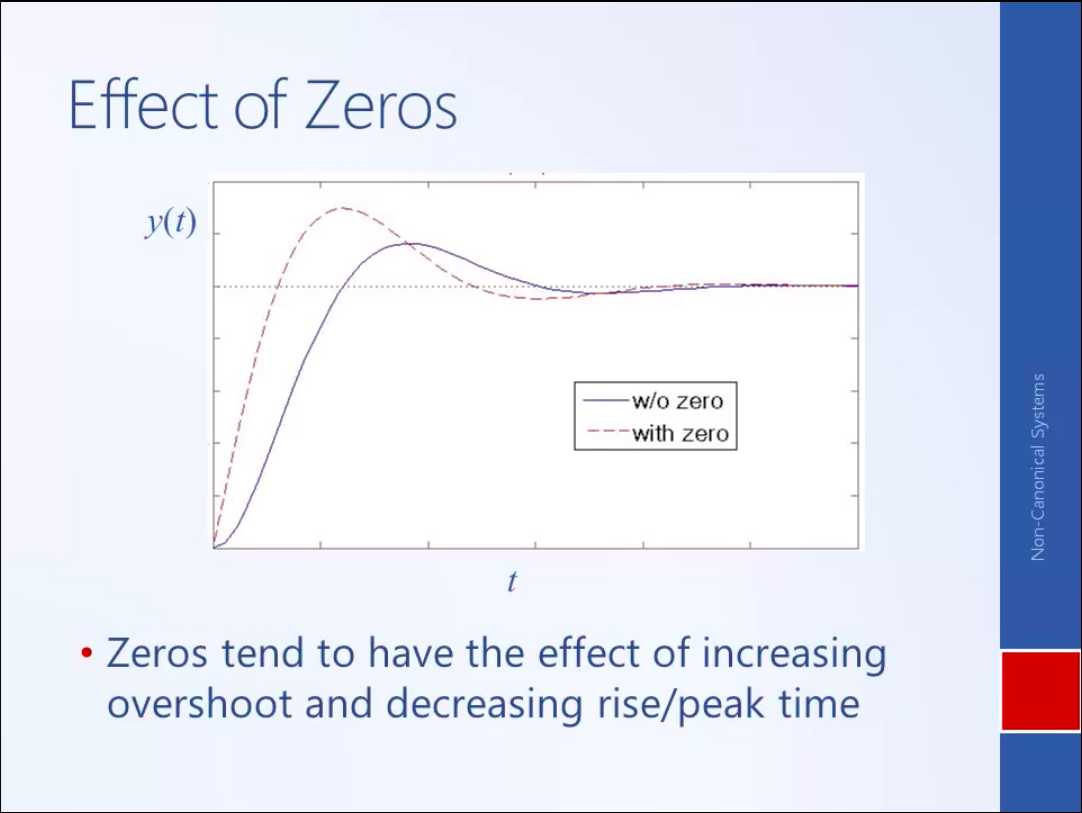
\includegraphics[width=\linewidth]{Bilder/EffectOfZeros2_2}
	\caption{Zeros increase the overshoot of the system}
	\label{Fig_EffectofZeros2_2}
\end{figure}
\clearpage
\subsubsection{Effect 3: Non-minimum Phase Behavior}
If the zero has a \textbf{\textit{positive real root}}, then it will induce into a system a response which will initially move in the reverse direction. Such a behavior is called a non-minimal phase behavior as exhibited by a bicycle when given an impulse torque to its steering.
\subsubsection{Effect 4: Canceling poles that are near them}
\begin{figure}[h!]
	\centering
	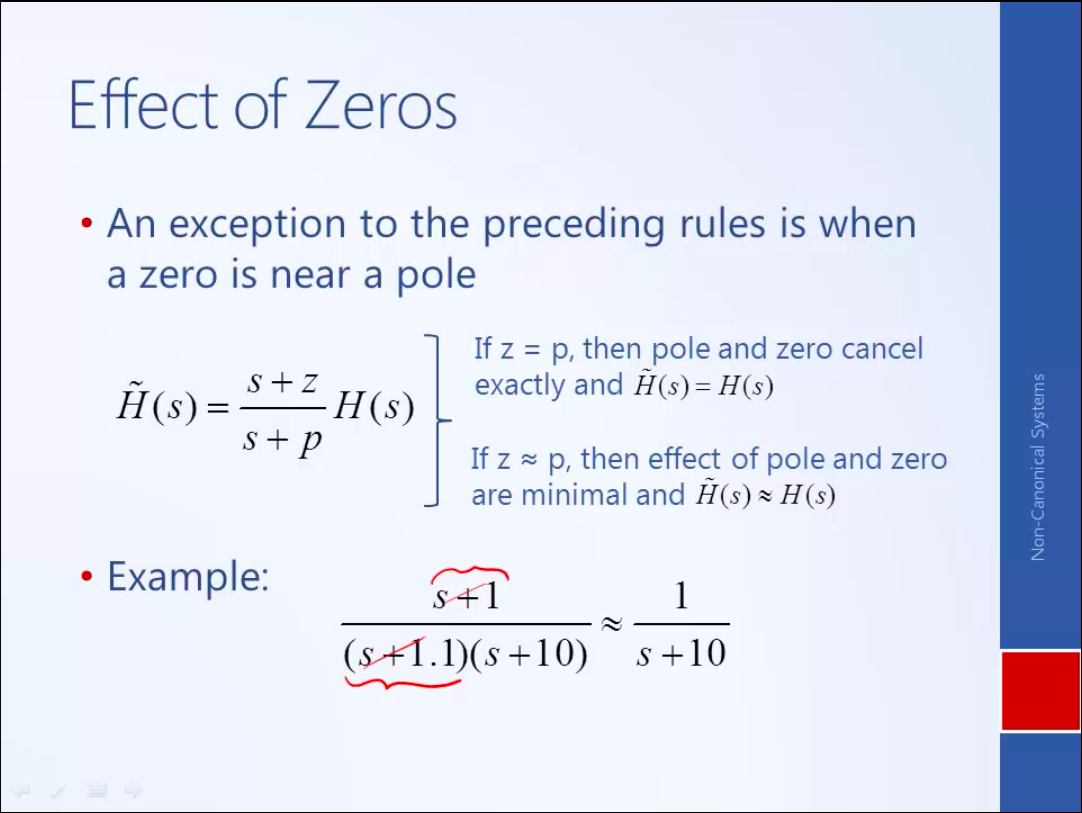
\includegraphics[width=\linewidth]{Bilder/EffectOfZeros4}
	\caption{Zeros which are close to poles cancel them}
	\label{Fig_EffectOfZeros4}
\end{figure}
\clearpage

\subsection{Nonlinear Systems}

In most of the cases the solution to the nonlinear systems are only possible numerically. Numerical approximation of the solutions do not yield the conceptual understanding that is possible with analytical solutions. One way to have an analytical solution is to use \textbf{\textit{Model reduction techniques}} in order to simplify (approximate) the nonlinear system into a linear system in a neighborhood about an operating point. Such as the linearinzing functions that are used around an operating point in mathematics. Which defines the approximation of a nonlinear function $f(x)$ about an OP $\bar{x}$:
\begin{equation}
	\frac{df}{dx} \approx \frac{f(x) - f(\bar{x})}{\Delta x}
\end{equation}
$f(x)$ is linearized using the above relation as:
\begin{equation}
	f(x) \approx f(\bar{x}) + \frac{df}{dx} \Delta x
\end{equation}
Lienarization is possible only near the small range of neighborhood just near the OP. As the system deviates from the OP the approximation made by the lienarization deviates rapidly. A more detialed analysis on linearization is shown in chapter \ref{Ch_Linerization}.













